%%%%%%%%%%%%%%%%%%%%%%%%%%%%%%%%%%%%%%%%%%%%%%%%%%%
\chapter{Trigonometria}

A trigonometria não é a ciência que mede os grãos de trigo, mas sim a ciência das sombras e das estrelas. Suas origens remontam a astronomia, agrimessura e as navegações.

Para Euclides (em sua obra chamada Elementos) foi dito que um ponto é algo que não tem dimensão ou parte alguma. A linha (em específico a reta) tem uma origem e uma extremidade que são pontos. A superfície corresponde corresponde a figura delimitada por linhas em sua borda. O plano é uma superfície que contem duas retas paralelas (ou concorrentes).

O círculo é uma figura interessante pois corresponde a superfície cujo todos os pontos de sua borda estão a mesma distância do seu centro. Além disso as linhas que ligam quaisquer dois pontos da borda do círculo é chamado de corda. A maior corda é a que passa pelo centro do círculo, ela é chamada de diametro do círculo. A metade do diametro é o raio.

\section{Contexto histórico}

O termo trigonometria significa a medida das partes de um triângulo.

Na grécia antiga temos estenços estudos entre os angulos (ou arcos) e as cordas em um mesmo círculo.

Hiparco foi chamado pai da trigonometria por ter desenvolvido cálculos precisos e com eles calcular a duração precisa do mês e do ano, o tamanho da luna e a precessão dos equinócios.

\section{Origem do termo seno}

Os árabes haviam traduzido textos de trigonometria do sânscrito. Os hindus tinham dado o nome de \textit{jiva} à metade da corda, e os árabes a transformaram em \textit{jiba}. Na língua árabe é comum escrever apenas as consoantes de uma palavra, deixando que o leitor acrescente mentalmente as vogais. Desse modo, os tradutores árabes registraram \textit{jb}. Na sua tradução do árabe para o latim, Robert de Chester interpretou \textit{jb} como as consoantes da palavra \textit{jaib}, que significa \textit{"baía"} ou \textit{"enseada"}, e escreveu \textit{sinus}, que é o equivalente em latim.\cite{eli1998trigonometric} e \cite{da2003historia} A partir daí, a \textit{jiba}, ou meia corda hindu passou a ser chamada de \textit{sinus}, e, em português, \textit{seno}.\footnote{\href{http://ecalculo.if.usp.br/historia/historia_trigonometria.htm}{Usp, Trigonometria}}

Uma das tarefas da astronomia foi o estabelecimento das tabelas. As primeiras tabelas, as de Hiparco, se perderam. Quanto às de Ptolomeu, estabeleciam as coorrespondências entre os comprimentos das cordas e dos diferentes valores de arcos.

Mais tarde os indianos substituíram as tabelas de cordas por tabelas de senos, mais fáceis manejar.


\begin{center}
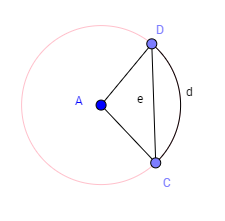
\includegraphics[scale=0.9]{./imagens/06.png}
\end{center}

\begin{center}
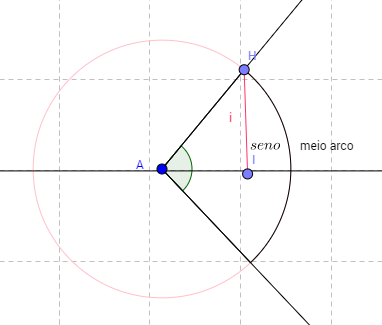
\includegraphics[scale=0.9]{./imagens/07.png}
\end{center}

A precisão de todo cálculo astronômico repousa na exatidão da tabela de senos, cuja construção está ligada ao problema da trisseção do ângulo! Al-Khuwarizmi foi o primeiro matemático árabe a estabelecer tabelas de senos! \cite{guedj2008teorema}

%\begin{center}
%\includegraphics[scale=0.9]{8.png}
%\end{center}
\section{Trigonometria no Triangulo Retângulo}

\begin{center}
%\scalebox{2}{
\begin{tikzpicture}
\coordinate[label=below left:$A$] (A) at (0,0);
\coordinate[label=below right:$B$] (B) at (4,0);
\coordinate[label=above right:$C$] (C) at (4,3);
\coordinate[label=below :cateto adjacente] () at (4/2,0);

\draw[thick] (B) -- (A) -- (C) -- (B);

\begin{scope}
\path[clip] (A) -- (B) -- (C);
\end{scope}

\draw[->] (0,0) ++(.5,0) arc (0:35:.5);
\draw[] (4,0) rectangle (3.5,0.5);

\node at (35/2:.8) {$\theta$};
\node[above,left] at (4/2,3/2) {hipotenusa};
\node[right] at (4,3/2) {cateto oposto}
%\node[above] at (4/2,0) {cateto adjacente}

\end{tikzpicture}
%}
\end{center}

\begin{table}[h]
 \centering
 \begin{tabular}{|c|c|}
 \hline
 seno & cosseno \\
 \hline
 $\sin \theta=\dfrac{C. op}{Hip}=\dfrac{a}{b}$ & $\cos \theta=\dfrac{C. ad}{Hip}=\dfrac{c}{b}$\\
 \hline
 \end{tabular}
 \caption{Seno e Cosseno no triângulo retângulo}
 \label{tab:my_label}
\end{table}


\section{Ângulo complementar e o Cosseno}
Dois ângulos são complementares quando sua soma dão um ângulo reto.

\begin{table}[h]
 \centering
 \begin{tabular}{|c|c|}
 \hline
 ângulo & complementar \\
 \hline
 0° & 90°\\
 \hline
 30° & 60°\\
 \hline
 45° & 45°\\
 \hline
 60° & 30°\\
 \hline
 90° & 0°\\
 \hline
 \theta & $90°-\theta$\\
 \hline
 \end{tabular}
 \caption{Ângulos complementares somados resutam um ângulo reto}
 \label{tab:my_label}
\end{table}

O cosseno é o seno do ângulo complementar. Ou seja, o cosseno de um ângulo é o seno do quanto falta para que esse ângulo se torne um ângulo reto.

\begin{table}[]
 \centering
 \begin{tabular}{|c|c|}
 \hline
 cosseno & seno \\
 \hline
 $\cos 0°$ & $\sin 90°$\\
 \hline
 $\cos 30°$ & $\sin 60°$\\
 \hline
 $\cos 45°$ & $\sin 45°$\\
 \hline
 $\cos 60°$ & $\sin 30°$\\
 \hline
 $ \cos 90°$ & $\sin 0°$\\
 \hline
 $\cos \theta$ & $\sin (90-\theta)$\\
 \hline
 \end{tabular}
 \caption{O Cosseno de um ângulo é o seno de seu complementar}
 \label{tab:my_label}
\end{table}
\newpage

\section{Ângulos Notáveis}
Os triângulos notáveis com que trabalhamos no Ensino Fundamental são $30^o, 45^o$ e $60^o$. No triângulo equilátero obteremos o seno e o cosseno de dois desses valores e com o quadrado de diagonal unitária o outro valor.

\subsection{$30^o$ e $60^o$}
É sabido que na Geomtria Euclidiana Plana o triângulo tem ao todo $180^o$ de ângulo interno. Em um triângulo equilátero temos, assim, três ângulos medindo $60^o$.
\begin{center}
\begin{tikzpicture}[scale=5]

\coordinate [label=below left:$A$] (A) at (0,0);
\coordinate [label=below left:$B$] (B) at (2,0);
\coordinate [label=above left:$C$] (C) at (1,1.71);
\coordinate [label=below left:$M$] (M) at (1,0);
\coordinate [label=below right:$N$] (N) at (0.9,0.1);
%\coordinate [label=below right:$h=\sqrt{3}/2$] (O) at (1,1.71/2);

\draw[thick] (B) -- (A) -- (C) -- (B);
\draw[thick] (C) -- (M);
\draw[thick] (M) rectangle (N);

\begin{scope}
\path[clip] (A) -- (B) -- (C);
\fill[red, opacity=0.5, draw=black] (A) circle (2mm);
\node at ($(A)+(30:3mm)$) {$60^o$};

\path[clip] (C) -- (A) -- (M);
\fill[blue, opacity=0.5, draw=black] (C) circle (2mm);
\node at ($(C)+(255:3mm)$) {$30^o$};
\end{scope}

\node[right] at (1,1.71/2) {$h=\frac{\sqrt{3}}{2}$};
\node[left] at (1/2,1.71/2) {$1$};
\node[below] at (1/2,0) {$\frac{1}{2}$};

\end{tikzpicture}
\end{center}
\section{Relação Fundamental da Trigonometria}

A relação fundamental da Trigonometria afirma que

\begin{equation}
    \sin^2 (\theta)+\cos^2 (\theta)=1
\end{equation}.

Isso é facilmente verificável para o triângulo retângulo cuja hipotenusa mede uma unidade como na imagem abaixo.

\begin{figure}[h]
    \centering
\scalebox{1}{
\begin{tikzpicture}[scale=1.00]
\coordinate[label=below left:$A$] (A) at (0,0);
\coordinate[label=below right:$B$] (B) at (4,0);
\coordinate[label=above right:$C$] (C) at (4,3);
\coordinate[label=below :$\cos (\theta)$] () at (4/2,0);

\draw[thick] (B) -- (A) -- (C) -- (B);

\begin{scope}
\path[clip] (A) -- (B) -- (C);
\end{scope}

\draw[->] (0,0) ++(.5,0) arc (0:35:.5);
\draw[] (4,0) rectangle (3.5,0.5);

\node at (35/2:.8) {$\theta$};
\node[above] at (4/2,3/2) {$1$};
\node[right] at (4,3/2) {$\sin (\theta)$}
%\node[above] at (4/2,0) {$\cos (\theta)$}

\end{tikzpicture}
}
    \caption{Triângulo Retângulo de hipotenusa medindo uma unidade}
    \label{fig:my_label}
\end{figure}



\begin{figure}[h]
    \centering
    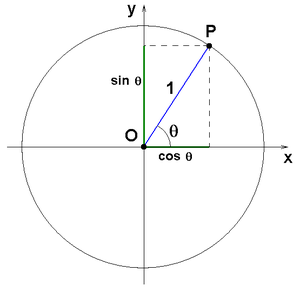
\includegraphics[scale=0.6]{./imagens/11.png}
    \caption{Círculo Trigonométrico de raio 1}
    \label{fig:my_label}
\end{figure}

\section{Seno e Cosseno da soma de arcos}



\section{Decomposição de Forças}

\begin{center}%Colocar alfa teta no lugar de alfa
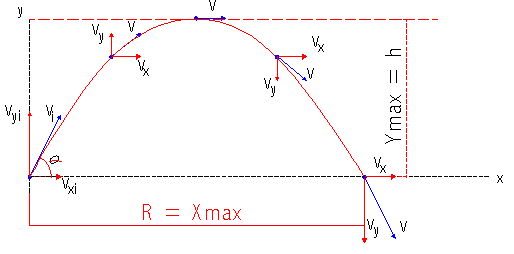
\includegraphics[scale=0.9]{./imagens/10.png}
\end{center}\\



$F=(F_x,F_y)=(F\cos \theta,F\sin \theta)$

